\documentclass[12pt, oneside]{book}
\usepackage[a4paper,top=2.5cm,bottom=2.5cm,left=3.5cm,right=2cm]{geometry}
\usepackage[utf8]{inputenc}
\usepackage[T1]{fontenc}
\usepackage{amsfonts}
\usepackage{graphicx}
\usepackage{url}
\usepackage[hidelinks,breaklinks]{hyperref}
\usepackage[english]{babel} % vypnite pre prace v anglictine
\usepackage{listings}
\usepackage{tikz}
\usetikzlibrary{automata,positioning}
\linespread{1.25} % hodnota 1.25 by mala zodpovedat 1.5 riadkovaniu

\lstset{
	basicstyle=\ttfamily,
}

% -------------------
% --- Definicia zakladnych pojmov
% --- Vyplnte podla vasho zadania
% -------------------
\def\mfrok{2018}
\def\mfnazov{Electronic Election System for Academic Senate}
\def\mftyp{Bachelor thesis}
\def\mfautor{Adam Štefunko}
\def\mfskolitel{RNDr. Jaroslav Janáček, PhD. }

%ak mate konzultanta, odkomentujte aj jeho meno na titulnom liste
\def\mfkonzultant{tit. Meno Priezvisko, tit. }  

\def\mfmiesto{Bratislava, \mfrok}

%aj cislo odboru je povinne a je podla studijneho odboru autora prace
\def\mfodbor{ 2508 Computer Science } 
\def\program{ Computer Science }
\def\mfpracovisko{ Department of Computer Science }

\begin{document}     
\frontmatter


% -------------------
% --- Obalka ------
% -------------------
\thispagestyle{empty}

\begin{center}
\sc\large
Comenius University in Bratislava\\
Faculty of Mathematics, Physics and Informatics

\vfill

{\LARGE\mfnazov}\\
\mftyp
\end{center}

\vfill

{\sc\large 
\noindent \mfrok\\
\mfautor
}

\eject % EOP i
% --- koniec obalky ----

% -------------------
% --- Titulný list
% -------------------

\thispagestyle{empty}
\noindent

\begin{center}
\sc  
\large
Comenius University in Bratislava\\
Faculty of Mathematics, Physics and Informatics

\vfill

{\LARGE\mfnazov}\\
\mftyp
\end{center}

\vfill

\noindent
\begin{tabular}{ll}
Study programme: & \program \\
Study field: & \mfodbor \\
Department: & \mfpracovisko \\
Supervisor: & \mfskolitel \\
% Konzultant: & \mfkonzultant \\
\end{tabular}

\vfill


\noindent \mfmiesto\\
\mfautor

\eject % EOP i


% --- Koniec titulnej strany


% -------------------
% --- Zadanie z AIS
% -------------------
% v tlačenej verzii s podpismi zainteresovaných osôb.
% v elektronickej verzii sa zverejňuje zadanie bez podpisov
\newpage 
\thispagestyle{empty}
\hspace{-4cm}
\includegraphics[width=1.3\textwidth]{images/zadanie_ENG}

\newpage 
\thispagestyle{empty}
\hspace{-4cm}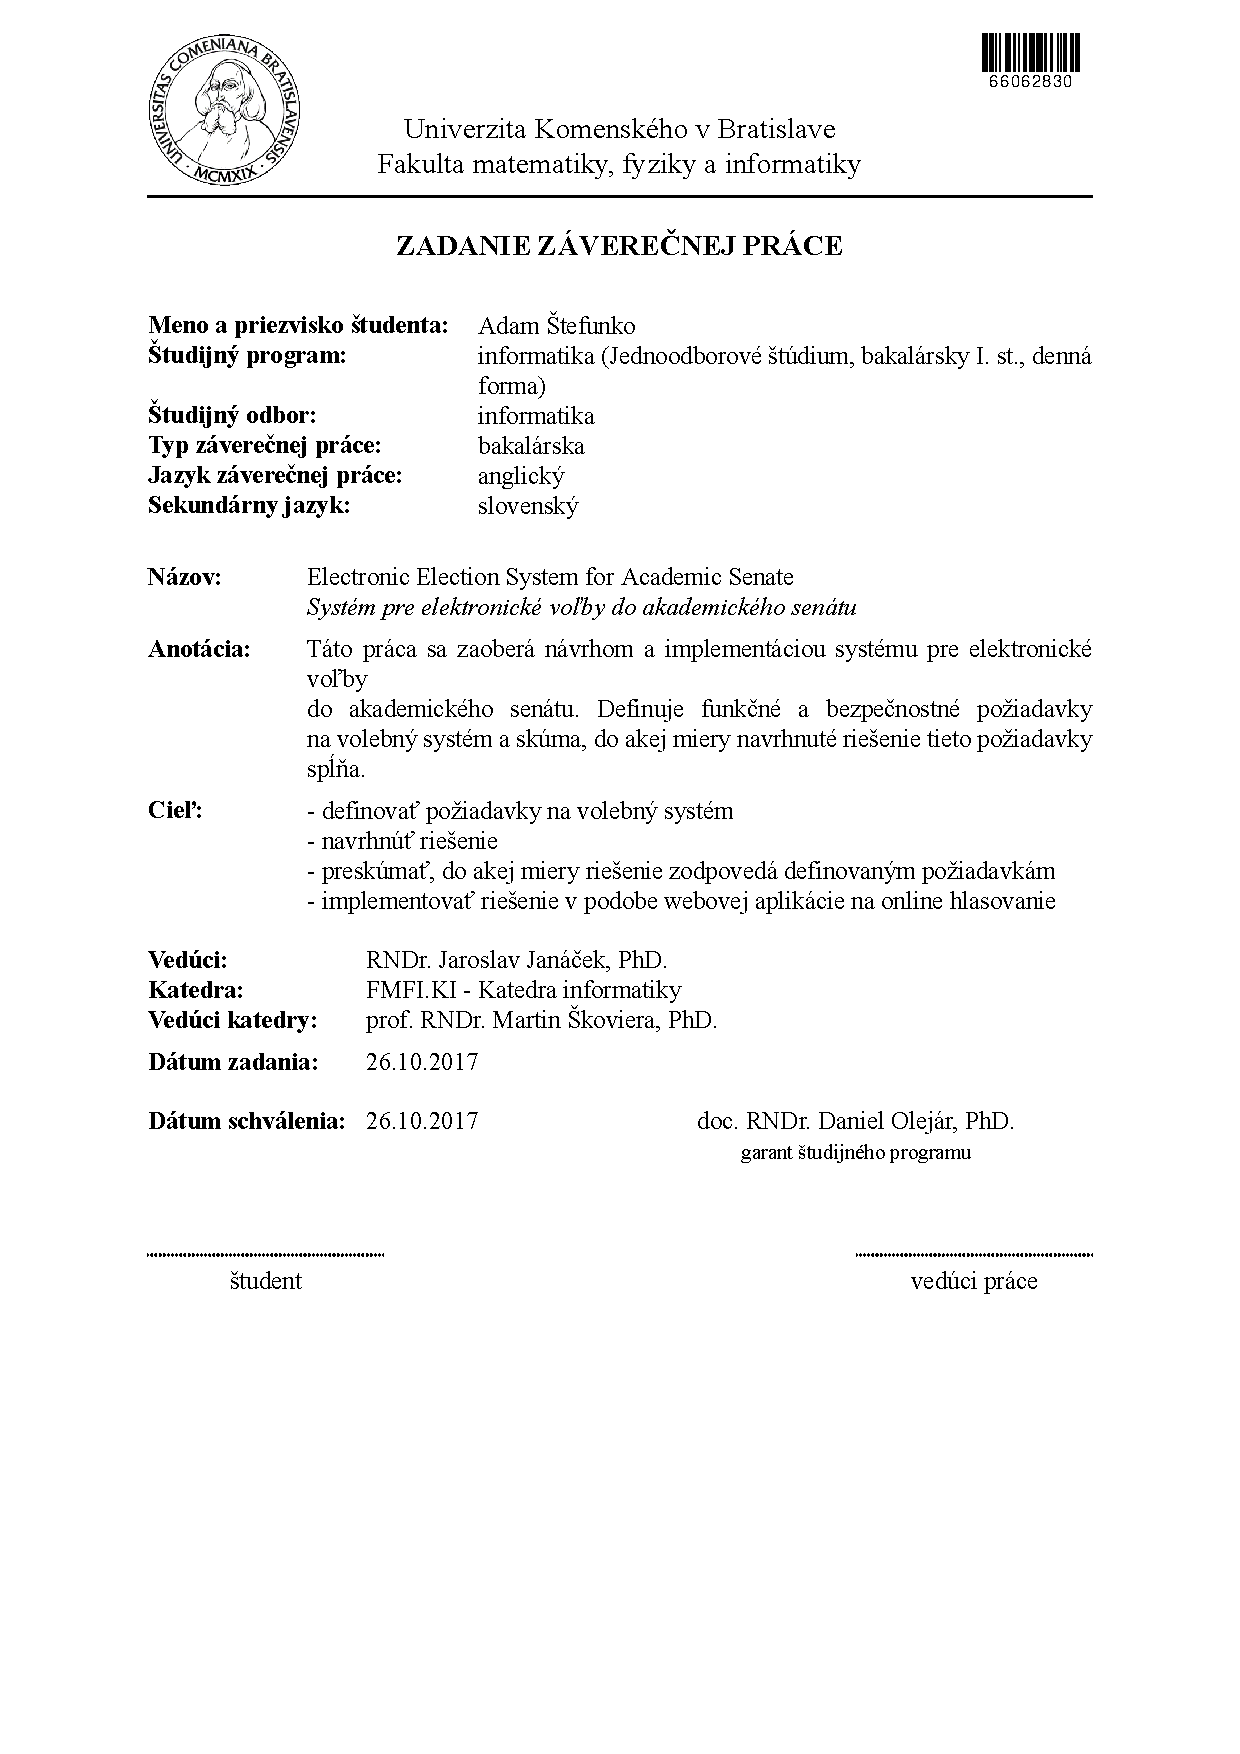
\includegraphics[width=1.3\textwidth]{images/zadanie_SVK}

% --- Koniec zadania

\frontmatter

% -------------------
%   Poďakovanie - nepovinné
% -------------------
\setcounter{page}{3}
\newpage 
~

\vfill
{\bf Acknowledgement:} 
There are many people to~which we want to~express our thanks. 

In~the~first place, we would like to~thank the supervisor of our bachelor thesis, \textbf{RNDr. Jaroslav Janáček, PhD.}, for~irreplaceable help and pieces of~advice in~various topics. These include design of~a~voting scheme or how to~correctly record our~thesis in~the~university's system. The~time we spent with him was very inspirational for~us.

A~few people quickly helped us with~several implementation problems. Thanks to~\textbf{Jakub~Šimo}, we discovered many \emph{JavaScript}'s secrets and we found~out why we were not able to install \emph{Python} packages on~our \emph{iMac}.

Our voting system is developed for~our faculty. Therefore, several faculty services needed to~be used within it. \textbf{Mgr.~Matej~Zagiba} explained to~us how \emph{Cosign} works and gave us numerous examples. \textbf{Bc.~Marek~Šuppa} gave us information about projects developed by the~members of~the~\emph{Student Development Team}.

Las but not least, we would like to~thank the~members of~\textbf{ŠKAS} (our faculty's student senate), and especially their vice-chair \textbf{Mgr.~Júlia~Pukancová}, for~suggesting us the~idea of~developing an~electronic election system for~our faculty.

% --- Koniec poďakovania

% -------------------
%   Abstrakt - Slovensky
% -------------------

% -------------------
% --- Abstrakt - Anglicky 
% -------------------
\newpage 
\section*{Abstract}

Electronic election represents a~modern way of~collaborative decision-making. It can, in~many aspects, simplify and automatise traditional election processes. However, it raises new security and usability questions. These include easy-to-use interface, cost-effectiveness, reliability of~the~system or correct computation of~the~votes. In~this thesis we try to~deal with~them and implement our own electronic election system. Inspired by~existing solutions, we propose our own electronic voting scheme. Our proposal is, then, used to~develop an~electronic election system. This system uses an~Internet browser to~cast a~vote and is run on~a~server, which also collects the~votes. At~the~end of~the~election process, the~votes are counted in~the~machine for vote counting. This system is developed on~top of~several cryptographic primitives, such as asymmetric encryption or secret sharing, which are also described in~this thesis. Our system is, finally, analysed regarding the~defined requirements.

\paragraph*{Keywords:} electronic election system, electronic voting scheme, internet application, academic senate

\newpage 
\section*{Abstrakt}


Elektronické voľby reprezentujú moderný spôsob skupinového rozhodovania sa. V~mnohom dokážu zjednodušiť a~zautomatizovať tradičné voľby, avšak prinášajú so~sebou nové bezpečnostné a~používateľské otázky. Sú to napríklad ľahko použiteľné užívateľské rozhranie, rentabilita, spoľahlivosť systému či~správne spočítanie hlasov. V~tejto práci sa s~nimi snažíme vyrovnať a implementovať náš vlastný elektronický volebný systém. Po inšpirovaní sa existujúcimi riešeniami navrhneme vlastnú elektronickú volebnú schéme. Z tejto schémy potom vyvinieme vlastný elektronický volebný systém. Tento systém využíva na~hlasovanie internetový prehliadač a beží na~serveri, ktorého úlohou je aj zbierať hlasy. Na~záver volieb sú hlasy sčítané v~sčítacom zariadení. Tento systém je postavený na~báze niekoľkých kryptografických metód, ako je napríklad asymetrické šifrovanie alebo zdieľanie tajomstva. Tieto sú taktiež popísané v~našej práci. Na~záver analyzujeme náš systém na~základe definovaných kritérií.
%Slovenský abstrakt v rozsahu 100-500 slov, jeden odstavec. Abstrakt
%stručne sumarizuje výsledky práce. Mal by byť pochopiteľný pre bežného
%informatika. Nemal by teda využívať skratky, termíny alebo označenie
%zavedené v práci, okrem tých, ktoré sú všeobecne známe.

\paragraph*{Kľúčové slová:} elektronický volebný systém, elektronická volebná schéma, internetová aplikácia, akademický senát
% --- Koniec Abstrakt - Slovensky


% --- Koniec Abstrakt - Anglicky

% -------------------
% --- Predhovor - v informatike sa zvacsa nepouziva
% -------------------
%\newpage 
%\thispagestyle{empty}
%
%\huge{Predhovor}
%\normalsize
%\newline
%Predhovor je všeobecná informácia o práci, obsahuje hlavnú charakteristiku práce 
%a okolnosti jej vzniku. Autor zdôvodní výber témy, stručne informuje o cieľoch 
%a význame práce, spomenie domáci a zahraničný kontext, komu je práca určená, 
%použité metódy, stav poznania; autor stručne charakterizuje svoj prístup a svoje 
%hľadisko. 
%
% --- Koniec Predhovor


% -------------------
% --- Obsah
% -------------------

\newpage 

\tableofcontents

% ---  Koniec Obsahu

% -------------------
% --- Zoznamy tabuliek, obrázkov - nepovinne
% -------------------

\newpage 

\listoffigures
%\listoftables

% ---  Koniec Zoznamov

\mainmatter


%\input uvod.tex 

%\input kapitola.tex

%\input latex.tex

%\input lorem.tex

%\input zaver.tex

\chapter*{Introduction}
\addcontentsline{toc}{chapter}{Introduction} % rucne pridanie do obsahu
\markboth{Introduction}{Introduction} % vyriesenie hlaviciek
This is the introduction to our bachelor thesis, introducing its important aspects.

\chapter{Description of~the~Electronic Election System}
\label{kap:definition}

In~this chapter, we talk about some possible definitions of~the~electronic election system, we propose a~definition with which we want to~work and we present some requirements on such a~system. We also discuss two main~approaches to~the~system in terms of technology used and describe our choice of~the~system we use for~our solution.

\section{Definition of~the~Electronic Election System}

\label{sec:def}

To~have the~system correctly and precisely designed, it is necessary to~have it clearly defined. At first, we need to~say something about the~electronic election or voting itself. We have borrowed descriptions from two large online encyclopaedias. We think they are amongst the~first sources to~which a~person being interested in~this particular topic is introduced. According to~Wikipedia, electronic voting "refers to~voting using electronic means to~either aid or take care of~the~chores of~casting and counting votes” \cite{Wiki}. In~comparison, Encyclopaedia~Britannica~offers this description of~electronic voting, "a~form of~computer-mediated voting, in~which voters make their selections with the~aid of~a~computer” \cite{Brit}. It can be observed that the~two descriptions are vague in~terms of~roles, or how the~actual voting and counting is processed. They only say that computers are used to~manipulate with the~votes and that voters are enabled to~vote using computers. For~the~use of~our thesis we define a~computer system which performs manipulation with the~votes and which is responsible for~the~electronic election. This is the~definition we propose:
\smallbreak
\textbf{Definition 1:} \emph{Electronic Election System} is a~computer system which
\begin{itemize}
\item[i.] authenticates the~voter,
\item[ii.] enables the~voter to~cast a~vote,
\item[iii.] securely transfers and stores the~vote,
\item[iv.] counts the votes.
\end{itemize}
\bigbreak
This definition simply enumerates all the~basic roles of~our electronic election system. We want the~election process to~be as automated as possible; therefore, the~definition is directly derived from the~tasks performed during regular election for~our academic senate. The~system authenticates a~voter, so it checks whether the~voter is authorised to~vote; it enables every authorised voter to~cast their vote; it transmits and stores every vote in~a~way that no vote is lost or changed; and after the~voting period has ended, it calculates all the~votes and outputs the~result.

%According to~Zuzana~Rjašková, "the~authorities and the~voters have to~follow electronic voting scheme" \cite{Rjaskova}. 
All the~authorities and voters involved in~electronic elections need to~follow a~particular electronic voting scheme (or protocol). This scheme prescribes procedures which should be proceeded during the~voting process and which should describe how the~electronic election system should perform its roles. 
%Rjašková \cite{Rjaskova} defines three stages of~which electronic voting scheme consists:
Such scheme usually consists of~three stages \cite{Rjaskova}:
\begin{enumerate}
\item \textbf{Initialisation}, during which the~elections are announced, questions are being made, and all the~private and public keys are being generated. 
\item \textbf{Voting}, during which voters are casting their votes: ballots are being created and then sent.
\item \textbf{Counting}, during which ballots are being opened and counted, and the~final results of~the~elections are being published.
\end{enumerate}

Several existing voting schemes are discussed in~Chapter \ref{kap:existing} and our proposed voting scheme is described in~Chapter \ref{kap:solution}.

\section{Requirements on an Electronic Election System}

\label{sec:requirements}

Every electronic election system must satisfy several requirements to~make sure that all its tasks have been performed unmistakably and that the~result is demonstrably correct. In~this section, we present several requirements which we find essential for~the~purposes of~the~elections to~the~academic senate. We also compare them to~the~requirements presented in~bibliography sources on this topic. %particularly with \cite{BunSri} and \cite{Rjaskova}.

P. P. Bungale and S. Sridhar from Johns Hopkins University, Baltimore have named several \emph{Requirements for~an Electronic Voting System} \cite{BunSri}. They have divided them into~two categories: "Functional Requirements" and "Security Requirements". We have chosen several of~them which we find most important for~our electronic election system, and we have added a~few that are not included in~Bungale's and Sridhar's original paper, yet we find them very important. We have partially followed their division. However, besides adapting the~terminology we have added an extra~category for~the~sake of~better distinction.  Thus, we divided them in~these three categories: \emph{usability}, \emph{security}, \emph{accuracy}. 
\bigbreak
Usability requirements are \emph{easy-to-use user interface}, \emph{mobility}, \emph{cost-effectiveness} and \emph{confirmation}.
\begin{itemize}
\item \textbf{Easy-to-use user interface.} The~system should have a~user interface which voters can use easily with (almost) no instructions provided. On top of~that, voting options should be displayed in~a~way that no candidate is disadvantaged.
%Also, as stated in~\cite{BunSri}, the~user interface "shall not disadvantage any candidate while displaying the~choices".
\item \textbf{Mobility.} The~voters should not be restricted to~a~certain~place where they can vote. In~terms~of~electronic voting, the~voter should not be limited to~a~certain~type of~technology used for~voting. In~spite of~Bungale's and Sridhar's opinion, who call voting via~the~Internet "\emph{infeasible} both for~security issues as well as social science issues" \cite{BunSri}, we advocate Internet voting because we think that in~certain~conditions, it is preferable and can meet our requirements (particularly this one).
\item \textbf{Cost-effectiveness.} The~technology used for~electronic voting should~not be expensive and hard to~implement, yet it must provide adequate functionality and security, so it can be effectively used as an electronic election system.
\item \textbf{Confirmation.} Each voter should have the~chance to~confirm that their vote corresponds to~their own decision and have the~chance to~modify their vote before committing it. Voters also should have the~chance to~verify whether their vote was correctly transferred and stored.
\end{itemize}

Security requirements are \emph{secrecy}, \emph{anonymity}, \emph{reliability} and \emph{incoercibility}.
\begin{itemize}
\item \textbf{Secrecy.} There must be no chance to~determine how a~voter voted.
\item \textbf{Anonymity.} No vote must be associated with a~voter's identity.
\item \textbf{Reliability.} The~system must be robust enough, so that no votes are lost or illegally changed in~any case, and it must be ensured there is no~malicious code or bugs. Also, the~system should be simple enough because such system offers fewer possibilities for~the~attackers and, thus, is less vulnerable.
\item \textbf{Incoercibility.} There must be no way in~which voter can prove how they have voted. This prevents from anyone else's impact on voter's choice and it also prevents from vote-selling.
\end{itemize}

Accuracy requirements are \emph{authorisation}, \emph{uniqueness and limitation}, \emph{persistence} and \emph{correct computation}.

\begin{itemize}
%\item \textbf{Eligibility.} "Only eligible voters can cast the~votes" \cite{Rjaskova}.
\item \textbf{Authorisation.} It must be secured that only authorised voters can cast their votes.
\item \textbf{Uniqueness and limitation.}  Each voter can participate in~an election by~no more than one vote and no~more candidates than allowed can be chosen.
%Each voter must not be allowed to~cast more than one vote
\item \textbf{Persistence.} It must be guaranteed that votes remain~intact after they have been committed and sent.
\item \textbf{Correct computation.} The~votes must be correctly computed according to the~published rules of~the~election.
\end{itemize}
For~comparison, Rjašková \cite{Rjaskova} has provided a~set of~seven requirements, which we introduce to~the~reader: \emph{eligibility}, \emph{privacy}, \emph{individual verifiability}, \emph{universal verifiability}, \emph{fairness}, \emph{robustness}, \emph{receipt-freeness}, \emph{incoercibility}. We strongly believe that almost each our requirement finds its counterpart in~one or more Rjašková's requirements, and vice versa. For~instance, counterpart to~confirmation is individual verifiability and counterpart to~reliability is robustness. Receipt-freeness means that there is no way to prove how a voter voted \cite{Delaune}. This can be substituted for incoercibility and vice versa.

\section{Types of~Electronic Election System}

%In~\ref{sec:requirements}, we have named several requirements that strongly influence how our system is developed. 
In~this section, we present two possible types of~electronic election system, which are the~most common, and of~which we choose one for~our purposes. Then, we compare those two types regarding our requirements which we presented in~Section \ref{sec:requirements}. We also present their advantages and their drawbacks. Finally, we give reasons for~our choice of~used type of~electronic election system.

Regarding the~technology used during the~voting phase (as described in~\ref{sec:def}), there are two main~types of~electronic election system: \emph{e-voting} and \emph{i-voting} \cite{Brit}.

\subsection{E-voting} 
This type uses special-purpose machines designed directly for~the~purposes of~the~elections. These machines either directly record the~ballots or they optically scan traditional paper ballots, which are then stored in~their internal memory. 

%"Assurance that the~vote is recorded as cast relies on testing of~the~machine’s hardware and software before the~election and confidence that the~software running during the~election is the~same software as the~one tested before the~election" \cite{Brit}. 
Reliability relies on testing the~machines during the~initialisation phase and on confidence that the~same software is running during the~whole election process. However, thanks to~relatively smaller number of~individual machines used during the~election and thanks to~higher possible responsibility from the~authority, these machines can be checked for~malicious software and controlled without much difficulty. Also, network communication between a~device of~this type and any other device is generally disabled. Hence, it is possible to~implement this type of~electronic election system in~a~way that it does not break security requirement in~such a~manner which is fatal to~the~election process. 

However, regarding functional requirements, we find this type of~system awkward. Firstly, special-purpose hardware is built to~hold the~tasks during the~election process and these machines are placed in~special-purpose polling stations where the~voting process is controlled by~a~commission. Voters have to~come to~the~polling station where they can cast their ballot. Depending on the~software in~these machines, it is possible that the~voter has to~learn how to~use the~machine before they cast their vote.

\subsection{I-voting}
The~second type, on the~other hand, uses Internet to~hold the~communication between the~authorities and the~voter that enables the~voter to~be authorised and to~cast their vote. 

One of~the~biggest security issues with this type of~the~system is the~relatively large amount of~independent devices, owned mainly by~the~voters themselves, which can run a~malicious software which might not, depending on the~security support of~the~individual device, be spotted. 
%As is written in~\cite{Brit}, "security experts worry that many personal computers are vulnerable to~penetration by~various types of~malware". 
Rubin~notes how many violent acts may potential attackers perform: "view every aspect of~the~voting procedure, intercept any action performed by~the~legitimate user with the~potential of~modifying it without the~user’s knowledge, and further install any other program of~the~attacker’s desire—even those written by~the~attacker—on the~voter’s machine" \cite{Rubin}.  The~second issue is the~Internet communication itself. Thus, cryptographic protocols, some of~which are to~be described particularly in~chapters \ref{kap:existing} and \ref{kap:solution} and~which are largely discussed in~\cite{Rjaskova}, are used to~prevent Internet communication from vulnerability during the~election process and to~assure to~a~great extent that security and accuracy requirements are not to~be broken.

Despite all the~security issues, mobility and cost-effectiveness are two important advantages of~this type of~electronic voting system. A~voter needs nothing, but their computer or mobile device with either a~special-purpose application or Internet browser. Moreover, it is relatively cheap to~develop a~special software that runs on a~user's device. There is left to~consider whether to~use Internet browser or a~special-purpose application. We find the~first option as preferable from the~point of~view of~mobility, whilst the~second is, in~our opinion, preferable when considering security. We should still bear in~mind that a~lot of~important details lie on the~way how the~system is developed, which is to~be discussed more deeply in~chapters \ref{kap:solution} and \ref{kap:implementation}.

\subsection{Comparison}

All these facts and expectations described above have been considered for~the~purposes of~our choice. We state that not all requirements we present in~Section \ref{sec:requirements} are equally important for~the~purposes of~the~system. Also, some requirements can be equally satisfied using either type. Mobility and cost-effectiveness have perhaps been the~most crucial during our decision process because our system is to~be made for~no more than a~thousand of~voters involved in~one election. Albeit not the~most secure, our system should provide reasonable security using accessible solutions. Some other security and functional requirements, such as anonymity, reliability and persistence, are essential, but these can be adequately achieved using either type of~the~system and appropriate protocols. 

E-voting systems are ideal for~elections involving a~large number of~voters, e.g. parliamentary elections, which is not our case. Thus, we decided to~use i-voting because it meets our functional requirements perfectly and it also provides adequate security thanks to~cryptography. Possible security issues can be treated quite quickly without any difficulty also thanks to~the~relatively small amount of~individuals involved in~the~elections.

%We have chosen i-voting for~the~purposes of~our electronic election system for~academic senate.
%E-voting systems are ideal for~large parliamentary elections, where 
%We would like to~create system which provides reasonable security using accessible solutions.






\chapter{Summary of~Existing Solutions}
\label{kap:existing}
Several computer scientists have been working on~electronic election systems until~this day. We introduce and describe some techniques used to~design electronic voting schemes as well as some existing solutions to~the~electronic elections. 

\section{Electronic Voting Scheme Techniques}

Electronic voting systems use several cryptographic primitives to~assure integrity, authenticity and correct transfer of~votes as well as to~preserve voter's anonymity. There are at least three specific techniques used to~design an~electronic voting scheme. These are \emph{blind signatures}, \emph{anonymous channels} and \emph{homomorphic encryption} \cite{Haenni}. They are used besides symmetric and asymmetric cryptography, certificates, digital signatures, etc. Here, we describe the~ideas on~which they are based and some of~their properties. We also briefly describe \emph{mixing networks}, \emph{onion~routing} and \emph{David Chaum's untraceable electronic cash protocol}.

\subsection{Blind Signatures}
In~many voting systems, blind signatures are used to~detach the~vote from~the~voter's identity. The~basic principle of~such schemes is that blinded empty ballot is sent to~the~authority alongside voter's personal information. After verifying voter's identity and correctness of~the~ballot, it is blind signed by~the~authority and sent back to~the~voter. Then, voter unblinds the~ballot, fills it and sends to~votes collector. Simple example of~such a~scheme is described in~\cite{Standford}.

As written in~\cite{Haenni}, all protocol requirements, except receipt-freeness, are accomplished in~schemes using blind signatures when some other cryptographic primitives, such as encryption, are used together with blind signatures. But, these schemes have restricted usability due to~the~fact that in~order to~ensure fairness and verifiability, voters need to~be active in~at least two phases. %In~\cite{Haenni} are also given examples of~protocols that overcome this functional drawback.
However, there are some protocols that overcome this functional drawback.
\subsection{Verifiable Anonymous Channels}
We use anonymous channels to~send anonymous messages. This means that there is no way to~trace the~received message back to~the~sender. Anonymous channels can~be built using \emph{mix networks} or \emph{onion~routing}. 
\begin{itemize}
\item \textbf{Mix Network} uses a~chain~of~proxy servers that mix the~multiple messages and send them in~a~random order to~the~next node, which might be either another mixing server or a~different type of~device.
\item \textbf{Onion~Routing} encapsulates a~message in~new layers of~encryption. Analogous to~this are layers of~onion, hence the~name. The~message is, then, transmitted through a~series of~subsequent routers, each decrypting the~actual top layer of~encryption~and uncovering the~message's next destination. In~every moment of~the~message transfer, only precedent and following location~is known to~each \emph{onion~router}, thus making the~sender's identity untraceable \cite{Goldschlag}.
\end{itemize}

It is necessary to~ensure that no messages are dropped or substituted during the~transfer. Therefore, \emph{proofs of~correct computation} need to~be provided. Channels that are able to~do so are called \emph{verifiable anonymous channels}. Their main~drawbacks are computational complexity and inefficiency \cite{Haenni}.


\subsection{Homomorphic Encryption} 
Use of~homomorphic encryption~is based on~the~desire to~decrypt the~sum of~votes without being able to~decrypt the~individual ballots. It means that no voter can get anyone else's vote, while the calculation of the votes remains publicly verifiable. For~that reason, voters can~openly authenticate to~the~server \cite{Katz}.

However, such schemes have several serious drawbacks. Not only do they require computationally intensive zero-knowledge proofs, but they also do not allow voter to~choose multiple options \cite{Haenni}.
\subsection{Untraceable Electronic Cash Protocol}
In~\cite{Chaum}, David Chaum introduces a~protocol which can~be used to~send electronic cash while preserving sender's anonymity and avoid double-spending at the~same moment. Moreover, if a~sender tries to~send several copies of~an~electronic coin, their identity can~be revealed. The~protocol also provides a~method that can~be used to~reveal double-spender's identity. With a~few modifications, this protocol is useful for~electronic voting to~prevent double-voting. % to~send a~vote and retain~the~same conditions. 

The~Chaum's protocol can~be described in~the~following way. It can~be noticed that we present only the~most important steps to~the~reader.
%("briefly described in~short sentences"):

In~this example, the~symbol $\cdot$ denotes concatenation. Let $n$ be an~RSA~modulus and let $f$ and $g$ be two-argument collision-free functions. Let $u$ be sender's account number and $v$ be a~counter associated with this number and kept in~the~bank.

\begin{enumerate}
\item{\textbf{Formation}
\smallbreak
\begin{enumerate}
\item The~sender chooses $k \in~\mathbb{N}$ values $a_i, c_i, d_i$ and $r_i$, where $1 \le i \le k$. All $a_i, c_i, d_i$ and $r_i$ are modulo $n$.
\item The~sender sends to~the~bank \emph{$k$ blinded candidates} $B_i = r_i^3f(x_i,y_i)\pmod n$, where $x_i = g(a_i,c_i)$ and $y_i = g(a_i \oplus (u\cdot (v+i)), d_i)$.
\item The~bank randomly picks $k/2$ indexes from~$\{i_1,...,i_k\}$.
%$\{i_j\}$, where $1 \le j \le k$, 
The~sender shows their $a_i, c_i, d_i$ and $r_i$ to~the~bank for~each picked $i$. From~these, the~electronic coin~$C$ is formed following steps described in~\cite{Chaum}.
\end{enumerate}}
\item{\textbf{Payment}
\smallbreak
\begin{enumerate}
\item In~order to~pay, the~sender sends their coin~$C$ to~the~shopkeeper.
\item{The~shopkeeper randomly chooses $k/2$ binary values $x_1, ..., x_{k/2}$. For~each $x_i \in~\{x_1, ..., x_{k/2}\}$:
\begin{itemize}
\item If $x_i = 0$, the~sender shows the~shopkeeper $a_i, c_i$ and $y_i$.
\item If $x_i = 1$, the~sender shows the~shopkeeper $a_i \oplus (u\cdot (v+i)), d_i$ and $x_i$.
\end{itemize}}
\item The~shopkeeper sends obtained values to~the~bank in~order to~verify the~coin~$C$.
\end{enumerate}
}
\end{enumerate}

When the~sender tries to~use $C$ twice, it can~be observed that with high probability complementary binary values will be sent to~the~bank for~at least one $x_i$ and the~sender's identity will be revealed. This is possible because in~this situation, all the~values $i$, $a_i$ and $a_i \oplus (u\cdot (v+i))$ are known, from~which the~sender's identity can~be easily extracted. 

Although not designed directly for~the~purposes of~electronic election, this protocol can~be used, requiring only slight modifications, such as making $u$ a~unique personal identification~number given to~every voter prior to~the~election. Such a~modified scheme can~be found in~\cite{Radwin}.
%Then, it can~be used for~the~purposes of~electronic elec
\section{Existing Electronic Election~Systems}
Many governments are interested in~replacing traditional election~schemes based on~paper voting with electronic election~systems. At the~turn of~the~millennia, \emph{SERVE} was an~ambitious experiment by~the~United States of~America~in~the~field of~Internet voting. It was later cancelled, mostly due to~large security weaknesses SERVE showed. Switzerland was amongst the~first countries to~use electronic elections in~some of~their cantons. Estonia~was the~first country to~run nationwide electronic parliamentary elections. In~this section, we describe pioneering election~systems developed for~Estonia, Norway and Switzerland.

\subsection{Estonian~Internet Voting}
Estonian~identification~cards (ID cards) have a~chip that stores asymmetric cryptography key pair, which their owners can~use to~digitally sign documents. This has been used to~develop an~internet voting protocol, which was first used during the~election~in~2005, while it was still possible to~vote traditionally. Information about~this protocol comes mainly from~\cite{Springall}. %Estonia~has launched dual voting. Electronic election~is enabled week before the~traditional election. Voter can~remotely change their opinion~as many times as they want, or they can~vote traditionally. 

The~protocol used in~Estonian~internet voting system uses method of~\emph{double envelope}. While the~outer envelope is used to~provide the~voter's identity, the~inner is used to~cryptographically protect the~vote. These entities play role in~this protocol: \emph{voter}, \emph{voting commission}, \emph{voting application}, \emph{server}, \emph{ballot box}, \emph{counting device} and \emph{certification~authority}. 
\bigbreak
The~protocol consists of~three stages, which we now describe: 
\begin{enumerate}
\item \textbf{Initialisation.} Election~asymmetric encryption~key pair is generated. The~public key is given to~every voter while the~private key is divided using a~secret-sharing scheme and each member of~voting commission~is given their piece. The~voting application~is digitally signed and provided to~every voter.
\item {\textbf{Voting.} Voter, who has validated their ID card, connects to~the~server and launches the~voting application~on~their device. In~order to~establish secure connection, the~voter needs to~provide a~PIN code associated with their ID card. The~voter, then, chooses their favourite options to~form the~vote. When the~vote is formed, it is padded using \emph{OAEP} padding scheme with randomness $r$ and encrypted with the~election~public key using \emph{RSA}. After that, the~voter digitally signs the~vote using their ID card. The~vote encryption forms the~lower envelope and assures the~vote protection, while the~digital signature forms the~upper envelope and identifies the voter. The~\emph{double-enveloped} vote is, finally, sent to~the~server. 

The~server verifies voter's identity and strips off the~upper envelope. It sends the~vote in~the~lower envelope to~the~ballot box and associates it with a~random token $t$. The~voter can~check whether their vote was correctly recorded using a~verification~app on~their smartphone. The~app reveals $r$ and $t$ in~the~form of~a~\emph{QR} code. The voter uses a~smartphone app to~scan the~\emph{QR} code and to~compare the~encrypted vote stored in~the~ballot box with a~simulated vote encrypted using $r$ and corresponding the~voter's choices. Verification can be done no later than half an hour after casting the vote and up to three times per a single vote.}
%It is worth mentioning here, the~every voter can~do these steps as many times as they want during the~election.
\item \textbf{Counting.} Valid encrypted votes stored (without the~signatures) in~the~ballot box are burned to~a~DVD, on~which they are transferred to~the~counting device. The~private key is reconstructed and loaded onto~the~counting device. It produces the~result, which is burned on~another DVD and published.
\end{enumerate}
\bigbreak
Estonia's Internet Voting Committee claim that, in~terms of~security and reliability, this voting protocol is equal to~traditional elections. However, it seems to~be controversial. Tests run by~a~team from~the~University of~Michigan~show that the~system can~be successfully attacked on~both the~client-side and the~server-side. In~one type of~client-side attacks we take advantage of~the~fact that the~voter can cast a~vote more than once. Malware is installed on~the~voter's computer that sniffs the~voter's PIN code while the~voter is electronically voting. The malicious program waits until~the~verification period expires or~until the~voting application is closed and the~\emph{QR} code can no~more be scanned. As~soon~as the~\emph{ID} card has been inserted into~the~computer, the~malware open a~hidden mock version of~the voting application and submits a~replacement vote  \cite{Springall}. 

\subsection{Norwegian~Internet Voting Protocol}
\label{sub:norwegian}
In~Norway, trial of~Internet elections was first organised in~2011. A~protocol that would satisfy the~security expectations was defined for~the~Norwegian~elections \cite{Gjosteen2010} and a~new cryptographic protocol was published two years later \cite{Gjosteen2012}. A~new instantiation~of~the~cryptosystem underlaying Internet voting in~Norway was introduced and is described in~\cite{Gjosteen2015}.

In~the~original paper, associated with the~election~in~2011, a~simplified voting protocol is described. We believe that this protocol provides enough information~about~the~ideas on~which the~Norwegian~internet voting is based. The~players in~the~protocol are: \emph{voter}, \emph{voter's computer}, \emph{ballot box}, \emph{receipt generator} and \emph{decryption~service}. 
\bigbreak
The~voting scheme is divided into~three stages and the~following steps are processed:
\begin{enumerate}
\item \textbf{Key generation.} %Secret values $a_1$, $a_2$ and $a_3$ are generated, such that $a_1 + a_2 \equiv a_3 \pmod q$, where $q$ is a~generated prime number. From~those values, public parameters $y_1$, $y_2$ and $y_3$ are computed. 
Asymmetric encryption~keys and three secret parameters for~the~election~are generated, first for~the~decryption~service, second for~the~ballot box and the~third for~the~receipt generator. From~these, associated public parameters are computed. Expected return codes for~each voter are also generated and sent to~the~voter.
\item \textbf{Voting.} When the~voter choses their options, voter's computer sends the~encrypted vote to~the~ballot box. With the~cooperation~of~receipt generator, receipt codes are generated and sent to~the~voter. Those are checked by~the~voter, if they correspond with the~expected receipt codes.
\item \textbf{Counting.} Submitted votes from~the~ballot box are sent to~the~decryption~device. There, they are decrypted and counted in~order to~get the~final result.
\end{enumerate}

According to~the~author of~the~protocol, its security properties are not perfect, yet it is reasonable to~be used for~an~i-voting experiment. In~order to~assure that the~vote remains confidential, the~voter's computer should not be corrupted. If the~vote is not correctly submitted, although not corrupted before being submitted, the~voter can~see this through receipt codes and can~complain. The~author also concludes that "any corrupt infrastructure player may prevent the~election~from~completing." \cite{Gjosteen2010}.

After the~elections in~2011, the~protocol used for~it was gradually renewed and improved. One of~the~last introduced improvements on~the~underlying cryptosystem was that new techniques were used to~prove the~knowledge of~the~decryption~of~the~encrypted text. These new techniques have the~same effect as former; however, due to~their use, the~underlying cryptosystem has a~better security proof~\cite{Gjosteen2015}.

\subsection{Swiss Online Voting Protocol}
There are multiple public voting events in~Switzerland every year. Not only can~the~citizens choose their representatives in~Federal Assembly, but also referenda~are organised federally or regionally. 

Cantons of~Geneva, Zürich and Neuchâtel were the~first to~introduce electronic voting. In~2013, The~Federal Council of~Switzerland published a~framework which provides security, verifiability and functionality requirements in~order to~allow all the~voters to~vote electronically. In~a~publication~by~Scytl \cite{Swiss}, a~protocol ensuring cast-as-intended verification~is provided. This protocol has been created on~the~basis of~Norwegian~internet voting protocol (described in~this thesis in~\ref{sub:norwegian}). It is basically the~improvement of~that protocol "by~not needing to~rely on~the~strong assumption~that two independent server-side entities do not collude to~preserve voter privacy" \cite{Swiss}. The~building blocks of~the~protocol are \emph{ElGamal assymetric encryption~scheme}, \emph{bit-length prime numbers} representing voting options, \emph{pseudo-random function~family}, \emph{signature scheme} made up of~probabilistic algorithms and a~\emph{verifiable mix network}.
\bigbreak
These are the~participants in~the~Swiss voting scheme:
\begin{itemize}
\item \textbf{Election~Authorities}, responsible for~the~whole elections;
\item \textbf{Voters}, who express their opinion~by~casting a~vote;
\item \textbf{Registration~Authorities}, who provide voters with all the~information~needed;
\item \textbf{Voting Server}, which receives, proceeds and stores the~votes;
\item \textbf{Voting Device}, responsible for~enabling the~voter to~select their options, forming the~vote and correctly send it to~the~voting server;
\item \textbf{Code Generator}, which generates return codes from~the~votes;
\item \textbf{Auditors}, in~charge of~verifying the~correctness and integrity of~election~process.
\end{itemize}
\bigbreak
The~Swiss voting scheme consists of~following processes divided into~four phases:
\begin{enumerate}
\item \textbf{Configuration.} A~set of~voters' identities $ID$ is defined and published. The~protocol uses several key pairs, of~which public keys are published. Those keys are \emph{election~public key}, \emph{ global code generation~public key}, \emph{signing public key}. Voting options are also published in~this phase. The~global code generation~private key is given to~the~code generator and the~registration~authorities, and the~signing private key is given only to~the~registration~authorities.
\item \textbf{Voter registration.} In~order to~register to~the~election, voter provides their identity $id \in~ID$ to~a~registration~authority. Then, voter is given their public and private keys, a~set of~return codes associated with particular choices and confirmation~and finalisation~codes. Also, voter's public key is published together with reference values associated with return codes and a~validity proof~for~finalisation~code.
\item{ \textbf{Voting.} When the~voter is successfully authenticated, voter's $id$ and public key are stored in~their voting device. The~voter votes by~choosing from~the~voting options and entering their private key. From~these, the~vote is created and sent together with voter's $id$ to~the~voting server. 

When the~server successfully receives the~vote and the~voter's identity, return codes are generated and shown to~the~voter, who, then, is asked to~confirm the~vote. The~voter does so by~providing their confirmation~code to~the~voting device. Subsequently, the~confirmation~message is sent to~the~server. When the~vote is confirmed and finalisation~code is sent back to~the~device and the~voter checks whether it matches the~finalisation~code they have obtained during the~registration.}
\item \textbf{Counting.} The~counting algorithm takes the~votes stored on~the~voting server, the~election~private key and validity proofs for~finalisation~codes and produces the~final result, which is, then, verified.
\end{enumerate}

The~described protocol requires the~voter to~type several private values to~the~voting device. This means to~copy by~hand 52 or 410 characters when \emph{Base32} is used \cite{Swiss}. The~voter cannot~perform such a~task. Therefore, the~protocol also describes a~usability layer, whose role is to~reduce the~length of~values that the~voter needs to~directly provide for~the~voting system. Its description~can~be read in~the~original paper a~we do not include it in~this thesis.





\chapter{Our Solution}
\label{kap:solution}
The~main purpose of~this chapter is to~present our own solution to~the~electronic election system. We describe players in~the~final voting scheme we implement, the~voting scheme itself and the~format in~which the~vote is stored and read. Then, we bring some description of~existing security schemes and services we use in~our solution. We also discuss some other proposals of~the~voting scheme, which we modified or rejected. 

\section{Our Voting Scheme}
Our voting scheme is similar to~the~scheme that has been developed for~elections in~Estonia. This scheme is described in~Chapter \ref{kap:existing}. Both schemes are based on~the~principle that voter's identity cannot be known to~any player besides that particular voter when their vote can~be decrypted or read. It means that computer that is responsible for~decrypting the~votes cannot obtain~any information about~any voter who casted their vote. 

We bear in~mind that we require the~voting process to~run in~an~Internet browser and that this technology has several limitations. The~reader can~read more about limitations of~the~technology used in~Chapter \ref{kap:implementation}.
%We bear in~mind that we require voting application to~be run in~an~Internet browser.

\section{Players in~Our Voting Scheme}
We shortly describe each player in~our voting scheme and their purpose.
\begin{itemize}
\item \textbf{Voter $V$} authenticates to~server for~vote collection $S$ using \emph{authentication authority $T$} and casts their vote using \emph{voting application $A$}. They also can~cast their vote in~paper form in~a~special-purpose room.
\item \textbf{Election commission $B$} are in~charge of~key generation during the~first phase. They hold secret key $SK$ generated for~\emph{machine for~vote counting $M$} and share corresponding public key $PK$. They also securely transfer encrypted data from \emph{server for~vote collection $S$} to~$M$. Data~can~be, then, decrypted using $SK$, provided to~$M$ by~$B$. In~the~end, they publish the~result of~the~elections. Last but not least, they are responsible for~paper votes casted in~a~special-purpose room designed for~the~elections.
\item \textbf{Database $D$} stores information about all the~candidates and identities of~all authorised voters. This information is then used by~$A$ and $S$ to~display list of~possible candidates and authorise \emph{voter $V$}. This database is physically stored on server $S$ and is accessible only to~$S$.
\item \textbf{Voting application $A$} provides user interface for~$V$ in~which they can~cast their vote. It also validates the~vote, converts it to~a~proper format and encrypts it using $PK$. Then it sends the~vote together with~the~voter's identity.
\item \textbf{Server for~vote collection $S$} receives encrypted vote and voter's identity and checks whether this identity corresponds to~any of~those stored in~\emph{database $D$}. If the~encrypted vote comes from~an~authorised voter, then it stores the~encrypted vote and the~voter's identity in~its internal database of~votes. This server also provides storage for~voting application $A$ and database $D$.
\item \textbf{Machine for~vote counting $M$} receives all the~votes (without identity of~any voter) stored in~$S$'s internal database and secret key $SK$. It, then, decrypts all the~received votes using $SK$, validates them and computes the~result of~the~elections, which is finally published. We point out that this machine is not connected to~any network prior or during the~elections. This machine is restricted to~be in~off-line mode until the~results of~the~elections are published. %and it is proved that the~election process has been correctly performed.
\item \textbf{Authentication authority $T$} is responsible for~authentication of~$V$ and provides $S$ with~$V$'s identity, which must \emph{1-to-1} correspond to~a~value in~$D$. For~purposes of~our voting scheme, we use \emph{Cosign}, which is a~service commonly used for~authentication of~students studying at our faculty. From~this point, we mean~\emph{Cosign} any time we talk about $T$. Similarly, we use term \emph{UK login} of~voter $V$ instead of~\emph{$V$'s identity}. More information about \emph{Cosign} is provided in~Section \ref{sek:cryptography}  and Chapter \ref{kap:implementation}.
\end{itemize}

\section{Phases of~Our Voting Scheme}
Our voting scheme is designed to~have three subsequent phases: \emph{initialisation phase}, \emph{voting phase} and \emph{counting phase}. The~basic purpose of~these stages is discussed in~chapter~\ref{kap:definition}. In~this section, we provide a~detailed description of~what is done during each of~these phases.

\subsection{Initialisation}
\begin{enumerate}
\item Database $D$ with~a~table of~candidates is created and stored on $S$. For~each candidate, the~table contains a~unique ID and name of~the~candidate.
\item A~table of~authorised voters is created in~$D$. For~each voter, this table contains their \emph{UK login}.
\item A~special \emph{UK login} is created for~the~election commission $B$. This login~is used when a~voter casts their paper vote.
\item Public key $PK$ and secret key $SK$ are generated. They are to~be used to~encrypt the~vote by~the~voting application $A$ and decrypt it by~the~machine for~vote counting $M$, respectively.
\item Using \emph{Shamir's Secret-Sharing Scheme}, the~key $SK$ is divided into~$n$ parts, where $n$ is the~number of~members of~$B$. The~key $SK$ can~be reconstructed from~any combination of~$k$ parts, where $k$ is the~smallest number of~members of~$B$ that have to~sign the~\emph{Protocol of~elections}. The~reader can~read more about the~scheme in~Section \ref{sek:cryptography}.
\item Public key $PK$ is shared with~all the~voters by~inserting it into~$A$ as a~constant value for~the~whole elections.
\end{enumerate}

\subsection{Voting}
%This phase follows after initialisation was completed. \smallbreak
For~each voter $V$:
\begin{enumerate}
\item Voter $V$ opens a~specific Internet location in~their browser and logs in~using $Cosign$ in~order to~authenticate to~$S$.
\item If $V$ is successfully authenticated, voting application is launched in~their Internet browser. This application contains a~form in~which there are three options for~each candidate.
\item When $V$ submits the~form, it is then validated regarding the~rules of~the~elections. When the~form is valid, vote in~the~format described in~Section \ref{sek:format} is created and this vote is encrypted using \emph{S/MIME} protocol and $PK$. Finally, the~vote and voter's \emph{UK login} are sent to~$S$ via~an~\emph{HTTPS} connection.
\item When $S$ receives the~encrypted vote, it compares the~sender's \emph{UK login} with~logins in~the~table of~authorised voters stored in~$D$. If it matches exactly one record, then it is compared whether there is a~record with~the~same login. If there already is such a~record and the vote in~this record is different form the~special \texttt{0} character vote in~$S$'s internal database of~votes, this vote is rewritten with~the~new one. If there is not such a record, the~login~and the~encrypted vote are stored in~the~database.
%then the~login~and the~encrypted vote are stored in~$S$'s internal database of~votes. If there already is a~record with~the~same login~and vote different form the~special \texttt{0} character vote in~the~internal database, the~former vote is rewritten with~the~new one.
\item If $V$ decides to~use paper vote and goes to~the~special-purpose voting room, the~election commission $B$ authenticate to~$S$ using their special \emph{UK login}. When they give $V$ a~ballot paper, they send a~special \texttt{0} character vote together with~$V$'s \emph{UK login}, which rewrites $V$'s electronic vote if they have sent one and prevents $V$ from~casting an~electronic vote.
\end{enumerate}

\begin{figure}
\begin{center}
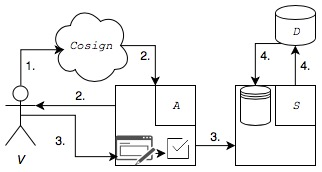
\includegraphics[scale=0.9]{images/Voting1}
\caption{Voting phase of~our scheme}
\end{center}
\end{figure}

\subsection{Counting}
\begin{enumerate}
\item Server $S$ is disconnected from~network and off-line mode is enabled.
\item Using a~secured USB device, the~election commission $B$ transfers encrypted votes from~$S$'s internal database of~votes to~machine for~vote counting $M$. It is crucial that \emph{UK logins} stored in~this database be excluded from~the~transfer.
\item With~aid of~at least $k$ members of~election commission $B$, secret key $SK$ is reconstructed. Then, it is inserted into~$M$ and used to~decrypt votes.
\item Decrypted votes are, then, validated by~$M$. All votes that are in~the~right format and follow the~rules of~the~elections are counted and the~final result is published.
\end{enumerate}

\begin{figure}
\begin{center}
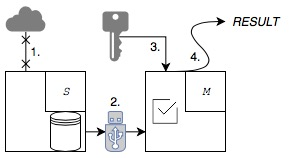
\includegraphics[scale=0.9]{images/Counting1}
\caption{Counting phase of~our scheme}
\end{center}
\end{figure}

\section{Format of~the~Vote}
\label{sek:format}
Definition of~format to~which each vote is formatted prior to~being sent to~the~server for~vote collection $S$ is also part of~our voting scheme. We want the~vote to~be stored in~one compact file and the~choices to~be clearly separated. It is known how many candidates are in~the~elections. Let $M$ be the~number of~candidates. Hence, we propose that the~vote is of~the~following format:
\begin{center}
\texttt{<candidate\_number\_1\#value\_1>...<candidate\_number\_M\#value\_M>}
\end{center}
Here, \texttt{M} is the~representation of~number of~candidates $M$.

This format represents a~string of~ordered pairs $(c_i, v_i)$, where $c_i \in~\{1,...,M\}$ is \newline \texttt{candidate\_number\_i} and $v_i \in~O$ is \texttt{value\_i}, $i\in~1,...,M$. Value $v_i$ is numerical representation of~one of~the~voting options and $O$ is the~set of~all possible numerical representations. For~example, 1 represents YES, 0 represents NO and $O = \{0, 1\}$. 

Let $(c_1, ..., c_M)$ be an~ordered set of~all candidate numbers. Then, $(c_1, ..., c_M)$ is a~permutation of~$\{1,...,M\}$.

It is obvious that the~candidate number 1, for~instance, is given YES if and only if the~vote contains exactly one ordered pair of~value $(1, 1)$.

\section{Security Tools Used in~Our Voting Scheme}
\label{sek:cryptography}
In~our voting scheme, we use these cryptographic protocols and schemes as well as security services to~securely transfer and store the~data.
\subsection{S/MIME}
Developed to~provide a~secure way to~send and receive MIME data, S/MIME (Secure/Multipurpose Internet Mail Extensions) consists of~several cryptographic services, such as authentication or data~encryption. Not only can~it be used by~traditional email clients but also by~message transfer services that use cryptographic solutions to~prevent any person from~undesired intervention. In~order to~use any of~the~services provided by~S/MIME, one must obtain~a~certificate from~a~certificate authority, which they then must install. S/MIME uses asymmetric cryptography based on \emph{PKCS\#7} standard.

%We use only data~encryption provided by~S/MIME. Therefore, we focus on describing this cryptographic service.

Ramsdell and Turner provide a~detailed specification of~S/MIME Version 3.2 in~\cite{Ramsdell}. More can~be also read in \cite{Turner} and \cite{SMIME}.
\subsection{Shamir's Secret-Sharing Scheme}
In~\cite{Shamir}, Adi Shamir proposes a~solution to~the~problem of~dividing data~into~$n$ pieces in~such a~way that these data~can~be reconstructed using $k$ of~these $n$ pieces, but attempt to~reconstruct the~data~with~fewer than~$k$ pieces results in~no information about it. Such a~scheme is called \emph{($n,k$)-threshold scheme}. The~scheme he proposed is based on polynomial interpolation. 

Let $p(x)$ be a~polynomial of~degree $d$. It is obvious that $d+1$ distinct points $(x_0, p(x_0)),...,(x_d, p(x_d))$ are sufficient to~define $p(x)$ and that $p(x)$ cannot be defined with~fewer than~$d+1$ distinct points. 
\bigbreak
In~Shamir's scheme, assume that data~$D$ is a~number. Then, to~divide $D$ into~$n$ pieces in~such a~way that it can~be reconstructed by~using at least $k$ pieces, we follow these steps:
\begin{enumerate}
\item We pick a~random $k-1$ degree polynomial $p(x) = a_0 + a_1x + ... + a_{k-1}x^{k_1}$, where $a_0 = D$. 
\item We, subsequently, evaluate $D_1 = p(1), ..., D_n = p(n)$. Then, each of~$n$ distinct pieces of~secret consists of~an~ordered pair $P_i = (i, D_i)$, where $i \in~1...n$.
\item In~order to~reconstruct data, at least $k$ pieces of~secret $P_{i_1}, ... , P_{i_k}$ are put together. Polynomial interpolation is then used to~find $p(x)$, which is the~Lagrange polynomial for~the~set of~used pieces of~secret. This makes recovering data~$D$ possible because $p(0) = a_0$ and $p(x)$ has been constructed in~such a~way that $a_0 = D$.
\end{enumerate}
The~scheme as described above consists only of~the~basic idea~on which secret sharing is based. In~reality, we use modular arithmetic instead of~its real counterpart. Let $p > \max(D, n)$ be a~prime number. Then, the~set of~integer coefficients $a_0, ..., a_{k-1}$ is picked randomly from~a~uniform distribution over integers in~$[0, p)$. Values $D_1, ..., D_n$ are also computed modulo $p$. The~set of~coefficients forms a~field $\mathbb{Z}_p$, which makes polynomial interpolation and data~retrieval possible \cite{Shamir}.

This scheme has some useful properties. It can~be observed that the~individual pieces are at most of the~same size as the~original data. With~$k$ fixed,  some pieces can~be added or deleted without affecting the~other, or the~pieces can~be changed without~changing the~original data. It is also possible to~reflect hierarchy in a~particular group, such as election commission, in a~way of distributing the~pieces. For~example, chairperson of the~commission is given three pieces, vice-chairperson two and the~other members one.
%By~solving a~system of~$k$ linear equations,  
\subsection{Cosign}
Comenius University in~Bratislava~uses \emph{Cosign}, a~secure single sign-on web authentication system originally developed at the~University of~Michigan~\cite{Cosign}. It is based on~web cookies. 

Authentication data~are sent to~the~central server, which uses an~authentication protocol to~verify these data. The~server, then, sets the~user a~web cookie, controlled by~\emph{Apache} filters during every user's attempt to~access addresses secured by~the~system. During the~whole process, \emph{TLS} is used for~a~secured communication.

In~Chapter \ref{kap:implementation} is described how authentication via~\emph{Cosign} has been integrated into~our system.
%\section{Accomplishment}
%In~this section, we discuss how our solution meets requirements.

\section{Other Proposed Solutions}
In~the~course of~designing the~final voting scheme for~our election system, we proposed some other solutions. Those were either rejected, or the~final scheme was based on them and their modifications.
There are two elementary design classes being in~consideration during the~whole process. Those are based on question whether server gives client any additional information used to~authorise the~sender of~the~vote. Regarding this, we consider two meaningful classes, which we call \emph{authorisation by~a~token} and \emph{authorisation~by~user information}. In~all of~the~schemes we have looked at, at~least three players represented by~computers are needed: a~\emph{client $C$}, an~\emph{authentication server $A$} and a~\emph{counting machine $B$}.

\subsection{Authorisation by~a~Token}
In~this design, authorisation in~provided~by~a~\emph{token}. This token assures $B$ that the~vote comes from~an~authorised voter without~associating it with~a~particular voter. In~order to~preserve anonymity, token must be generated or handled with~in~a~way that it cannot be associated with~any particular voter. In~Chapter \ref{kap:existing}, we describe some existing solutions using this design. 

Here, we briefly describe voting phase of~a~scheme that uses server $A$'s signature to~prove that the~vote comes from~an~authorised voter. 
\bigbreak
Let $V$ be voter and $n \in~\mathbb{N}$, $n \ge 2$, be constant defined by~the~scheme. Then, for~each voter $V$:
\begin{enumerate}
\item Voter $V$ logs~in~and voting application is opened on $C$.
\item Client $C$ sends $n$ encrypted votes and $V$'s identity to~$A$, where 1 of~those is the~real vote and the~other votes are fake.
\item If $V$ is an~authorised voter, $A$ signs all $n$ votes and sends them back to~$C$.
\item Client $C$ sends the~signed real vote to~$B$.
\item Server $B$ validates the~vote and if it recognises the~signature with~which the~vote is signed, then it stores the~vote.
\end{enumerate}

The~main~issue with~this scheme is that it may enable the~voter to~double-vote when their voting application is corrupted. In~Chapter \ref{kap:existing} we introduce the~reader to~David Chaum's scheme, which was designed to~be used with~electronic cash to~prevent double-spending. When using a~modification of~this scheme to~prevent double-voting, we face a~problem. In~order to~achieve this, additional data~about the~voter have to~be generated and stored on client's side. Of~course, these data~cannot be stored on voter's personal computer or smartphone, since our scheme is supposed to~be mobile and these data~have to~be accessed from~any device of~those kinds. This means that a~cloud storage in~which these data~can~be stored has to~be provided. This storage has to~be secured in~a~way that only voter can~freely access the~data. It raises new security tasks, which we think the~reader can~imagine. We do not say that it is impossible to~implement such a~system, but we think that it is not necessary to~implement such a~complex system for~purposes of~our type of~elections.

We have also come up with~a~totally different scheme using mix networks, referred to~in~Chapter \ref{kap:existing}, to~mix the~tokens in~order to~assure anonymity.

\begin{figure}[h]
\begin{center}
%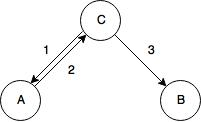
\includegraphics{images/PE2}
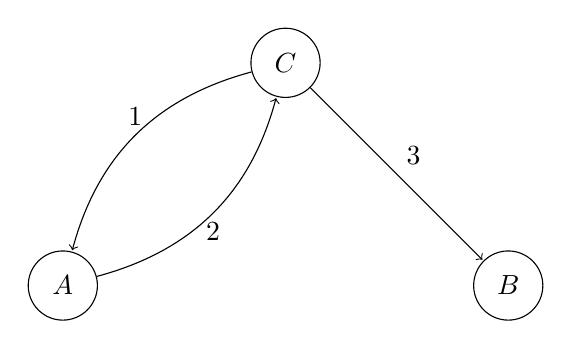
\begin{tikzpicture}[shorten >=0.5pt,node distance=4cm,on grid,auto] 
   \node[state] (A)   {$A$}; 
   \node[state] (C) [above right=of A] {$C$}; 
   \node[state] (B) [below right=of C] {$B$}; 
    \path[->] 
    (A) edge[below, bend right]  node {2} (C)
    (C) edge[above, bend right]  node {1} (A)
    (C) edge  node  {3} (B);
\end{tikzpicture}
\caption{Authorisation by~a~token}
\end{center}
\end{figure}

\subsection{Authorisation by~User Information}
Using voting schemes in~this class, $C$ assures that the~vote comes from~an~authorised voter by~providing a~publicly inaccessible piece of~information unique for~that voter that can~be matched with~a~record in~$A$'s memory. In~order to~retain~anonymity, the~vote must be in~an~illegible form during the~whole time it can~be associated with~this piece of~information.

Here, we provide a~simple scheme that has been modified and partly used in~the~final voting scheme.
\bigbreak
Let $V$ be voter. Then, for~each voter $V$:
\begin{enumerate}
\item Voter $V$ logs in~and the~voting application is opened on $C$.
\item Client $C$ sends encrypted vote and $V$'s identity to~$A$.
\item If $V$ is authorised to~vote, then $A$ sends the~encrypted vote without $V$'s identity to~$B$.
\item Server $B$ stores the~vote. 
\end{enumerate}
This scheme has several security issues. Let corrupted $A$ send $B$ encrypted votes and voters' identities. These votes can~be, then, decrypted by~$B$, which also knows who casted which vote. Thus, it can~be revealed how voters voted.

Due to~this fact, we propose in~our final solution that the~server $A$ stores the~votes in~an encrypted form and that the~device $B$ stays in~off-line mode during~the~whole election. Moreover, the~server $A$ is turned off before the~votes are provided to~$B$. This disables all the~possible communication between $A$ and $B$. We only need to~assure that nothing but~individual encrypted votes are transferred from~$A$ to~$B$ by~the~election commission.
\begin{figure}[h]
\begin{center}
%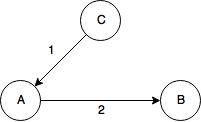
\includegraphics{images/PE1}
\begin{tikzpicture}[shorten >=0.5pt,node distance=4cm,on grid,auto] 
   \node[state] (A)   {$A$}; 
   \node[state] (C) [above right=of A] {$C$}; 
   \node[state] (B) [below right=of C] {$B$}; 
    \path[->] 
    (C) edge[above]  node {1} (A)
    (A) edge[below]  node  {2} (B);
\end{tikzpicture}
\caption{Authorisation by~user information}
\end{center}
\end{figure}












\chapter{Implementation of~Our Solution}
\label{kap:implementation}
Our task for this thesis is to develop a functioning electronic election system that can be used by our faculty's academic senate. In this chapter, we describe some important implementation details and we provide examples of important parts of our code.

\section{Overview}
For the desired system, we implement the electronic voting scheme described in chapter \ref{kap:solution}. This scheme consists of several entities, which together make our election system and some of which are represented by computers. Such \emph{players} have to be implemented independently, each running its own program that provides all its functionality and communication with other entities. Analysis of the final solution can be found in chapter \ref{kap:analysis}.

We have chosen \emph{Python} and \emph{JavaScript} as our primary programming languages. For databases, we use \emph{SQL}, a standard language in database programming.

In order to run the system correctly, there have to be some technical requirements accomplished. On the client-side, the voter needs to have one of these supported Internet browsers: \emph{Mozilla Firefox}, \emph{Google Chrome} or \emph{Safari}. The system is developed to run on \emph{Linux} distributions and the system can be build from existing Python files. In order to provide the authentication, the server needs to have $Apache 2$ server installed with a module that provide CoSign functionality. More can be read on webpages of our faculty.
\section{Database}
\section{Voting Application}
\section{Server for Vote Collection}
\section{Machine for Vote Counting}
\section{Supplementary Programs}

\chapter{Analysis of~Our Solution}
\label{kap:analysis}

%In~this chapter, we discuss how our solution~meets requirements established in~chapter \ref{kap:definition}.
In~Chapter \ref{kap:definition}, we established several requirements concerning \emph{usability}, \emph{security} and \emph{accuracy} of~an~electronic election~system. In~this chapter we briefly and informally analyse how our solution~presented in~Chapters \ref{kap:solution} and \ref{kap:implementation} meets these requirements.

\section{Usability}
Here, we discuss the~usability of~our electronic voting system concerning these points:
\begin{itemize}
\item \textbf{Easy-to-use user interface.} Our user interface is provided by an~online application. Users can~easily log in~using the~usual method used by our faculty. The~actual voting is done by clicking on~a~few radio buttons and clicking on~two submit buttons. The~voter is given the~information~on~the~number of~candidates they can~vote in~favour of. On~the~other hand, we could say that~giving answer for~every candidate might be time consuming. But, the~\emph{neutral} option~is set as the~default option. It means that~the~voting time can~be reduced just to~giving \emph{yes} answers to~the~desired candidates while the~others are left with the~default answer.
\item \textbf{Mobility.} The~voter is not restricted to~a~particular type of~device, nor have they to~stick on~an~individual device. What~is more, no voting application~is needed to~be installed. The~voters can~access voting everywhere. The~only thing they need is a~device with a~supported Internet browser and an~Internet connection.
\item \textbf{Cost-effectiveness.} The~system requires two to~three computer devices on the~server side, which can~be costly depending on~the~resources of~the~faculty. Yet, all the~software used for~the~system is open-source, so that~it does not require any additional financial resources.
\item \textbf{Confirmation.} When the~vote is formed, the~voter can~still change their mind and create another vote before~the~former would be sent. Moreover, using the~electronic voting, the~voter can~cast a~vote as many times as they want to~and only the~most current one remains recorded. Yet, confirmation~is not fully implemented in~our solution. For~example, the~Estonian~voting protocol, described in~Chapter \ref{kap:existing}, implements an~application~that~the~voter can~use to~check their vote. It might be possible to~implement such an~application~for~our electronic election~system, too. However, this is not included in~our implementation~partly due to~preserving \emph{incoercibility}.
\end{itemize}
\section{Security}
In~this section, we discuss how secure our solution~is. We analyse these requirements:
\begin{itemize}
\item \textbf{Secrecy and anonymity.} When the~vote is formed and sent to~the~server for~vote collection, it is in~an~encrypted state and the~server does not possess~the~election~private key, which must be used to~decrypt the~votes. Instead, this private key is shared among members of~the~voting commission, using a~secret-sharing scheme. When the~votes are transferred to~the~machine for~vote counting, they are no more associated with voters' identities. Therefore, they can~be decrypted and counted there. Keeping secrecy and anonymity relies mostly on~the~election~commission. They should not provide the~server for~vote collection~with the~election~private key. They must not provide the~machine for~vote counting with voters' identities associated with the~votes, either. The~most vulnerable part of~our code is retrieving the~encrypted votes from~the~database of~votes and saving them to~the~USB flash drive. At~this very moment, a~bug or undesired intervention~can~cause lost of~secrecy and anonymity.
\item \textbf{Reliability.} Our voting scheme is very minimal and mostly uses known techniques. Votes are stored in~a~database and associated with an~individual identity for~most of~the~time. No anonymous channels, described in~Chapter \ref{kap:existing}, are used. Therefore, chances that~the~votes are dropped or substituted while they are transferred or stored are low. Moreover, a~suspicious voter can~cast their vote again~if they think there is chance that~is has not been recorded correctly. Reliability also rests on~the~election~commission~during administration~of~paper voting and during the~maintenance of~server-side devices used. On~the~other hand, voters are responsible for~they devices and they can~contain~malware, which can~affect the~election. Our implementation~relies on~at~least two cryptographic libraries. It means that~there can~be some bugs in~them, as well. If we find that~out, we are ready to~update our implementation~according to~the~findings. 
\item \textbf{Incoercibility.} The~voter can~change their vote in~any moment. That~means that, from~the~client side, there is no such a~way in~which the~voter can~prove how they voted most recently. On~the~other hand, the~encrypted votes are stored together with \emph{UK login}s of~the~voters' and the~voters have access to~the~encrypted vote stored in~their Internet browser during the~voting session. %If an~attacker succeeds in~accessing the~database of~votes, they can~use comparable methods to~check how an~individual voted when they have access to~the~encrypted vote from~the~individual's Internet browser.
If an~attacker succeeds in~accessing the~database of~votes, they can~compare the~encrypted voter's vote in~the~database with the~encrypted vote from~the~voter's Internet browser.
\end{itemize}
\section{Accuracy}
It is important to~make sure that~only valid votes are recorded, all the~votes are accurately counted and the~right result is displayed. Now, we discuss how our solution~meets our accuracy requirements:
\begin{itemize}
\item \textbf{Authorisation.} In~our system, voters are authorised twice. First, they need to~log in~using \emph{Cosing}, an~authentication~system used by our University, before~the~voting application~is even displayed to~them. When they send their vote together with their identity provided by \emph{Cosign}, the~server for~vote collection~checks whether they are allowed to~vote. If not, the~sent vote is, simply, not recorded. %This means that~only students of~our University have access to~the~voting application.
\item \textbf{Uniqueness and limitation.} Every voter participating in~the~electronic election~is allowed to~cast as many votes as they want to. However, only the~most recent vote remains recorded. As soon~as they participate in~the~paper election, their electronic votes are erased and they are not able to~participate in~the~election~anymore. The~voting application~checks whether the~voter does not vote for~more than~allowed number of~candidates in~a~single vote. Due to~the~fact that~the~code of~the~voting application~can~be changed in~the~Internet browser and an~invalid vote can~be sent, this is double-checked during the~counting phase of~our election~system.
\item \textbf{Persistence.} Sent votes are stored in~the~database and handled with according to~the~voting scheme. They are transferred only once—from~the~server for~vote collection~to~the~machine for~vote counting. However, the~votes can~be irreversibly changed by the~election~commission~if they accidentally make a~record about a~voter that~has not been involved in~paper voting, yet.
\item \textbf{Correct computation.} The~machine for~vote counting is responsible for~the~correct computation. Therefore, this depends on~the~correctness of~the~particular implementation~of~the~machine for~vote counting. We have not discovered any bugs regarding vote computation~in~our implementation.
\end{itemize}

\chapter*{Conclusion}
\addcontentsline{toc}{chapter}{Conclusion} % rucne pridanie do obsahu
\markboth{Conclusion}{Conclusion} % vyriesenie hlaviciek
%This is the~conclusion of~our bachelor thesis, summarising its important points.
%Electronic elections have become integral part of~governmental administration in~Estonia, Norway and Switzerland and 
Estonia Norway and Switzerland are piloting countries in~developing and organising electronic elections. Their election systems represent reasonable solutions and use several cryptographic primitives to~provide enough security and reliability. Representatives of~our faculty also expressed interest in~electronic elections as a~tool of~democracy for~our students and this thesis deals with~this desire.

Firstly, we defined the~electronic election system and its three basic phases, and we presented some usability, security and accuracy requirements. This was important because we needed to~describe the~topic with~which we were about to~deal as clearly as possible. Keeping in~mind these requirements, we also discussed two main types of~electronic election system in~terms of~their functionality.

%remote electronic election
We also gave examples of~existing systems and described technologies they used in~order to~retain all the~aspects of~a~secure and reliable electronic election system. We also discussed some problems that those systems had. 

This led us to~our own proposal of~the~electronic election system. We listed players in~this system, including voters or vote counting machine. These players played several roles in~three phases of~our proposed voting scheme. This scheme uses several technologies, such as \emph{secret-sharing scheme}, \emph{Cosign} authentication system and \emph{S/MIME} encryption standard. To~provide the~reader with~some information on~how our system had been designed, we described several proposed schemes and we explained to~the~reader why we either rejected them or built on~top of~them.

As part of~our this thesis, we also implemented the~proposed system as an~Internet application. This included implementation of~the~voting application, which can run in~the~Internet browser, server for~vote collection, machine for~counting the~votes and some supplementary administration programs. 

Finally, we analysed our system regarding the~usability, security and accuracy requirements we defined.

We must admit that we met challenges of~various kinds during the~implementation of~our system. In~the~first place, we needed to~learn how to~work with~various cryptographic libraries, particularly \texttt{M2Crypto} for~\emph{Python} and \emph{PKI.js} for~\emph{JavaScript}. We were not a~hundred percent successful in~using these libraries, but we think that we managed to~create a~reasonable implementation. We also learnt a~lot about the~work with~\emph{CGI} scripts and \emph{S/MIME} encryption. Although we possessed a~theoretical basis in~those topics, we needed to~learn from~scratch how to~practically use them in~order to~create a~working system. Last but not least, we learnt new information about the~Internet infrastructure of~our faculty and how to~use \emph{Cosign}, a~secure single sign-on used by~our university.

We hope that this thesis represents only the~beginning of~this electronic election system. There are several other goals that we want to~be accomplished. First, the~system needs to~be deployed and tested in~the~environment of~our faculty. Then, it can be improved and extended. A~smartphone application can be one of~such extensions. We think there is a~lot to~do in~the~system itself, as well. For~example, key generation and customisable answers is something we have not implemented, yet. And last but not least, our system must be used during a~real election in~order to~find out all its advantages and drawbacks and to~figure out to~what extent we accomplished all our desires.

% -------------------
% --- Bibliografia
% -------------------


\newpage	

\backmatter

\thispagestyle{empty}
%\nocite{*}
\clearpage

\bibliographystyle{plain}
%\bibliography{literatura} 
\bibliography{bibliography}

%Prípadne môžete napísať literatúru priamo tu
%\begin{thebibliography}{5}
 
%\bibitem{br1} MOLINA H. G. - ULLMAN J. D. - WIDOM J., 2002, Database Systems, Upper Saddle River : Prentice-Hall, 2002, 1119 s., Pearson International edition, 0-13-098043-9

%\bibitem{br2} MOLINA H. G. - ULLMAN J. D. - WIDOM J., 2000 , Databasse System implementation, New Jersey : Prentice-Hall, 2000, 653s., ???

%\bibitem{br3} ULLMAN J. D. - WIDOM J., 1997, A First Course in Database Systems, New Jersey : Prentice-Hall, 1997, 470s., 

%\bibitem{br4} PREFUSE, 2007, The Prefuse visualization toolkit,  [online] Dostupné na internete: <http://prefuse.org/>

%\bibitem{br5} PREFUSE Forum, Sourceforge - Prefuse Forum,  [online] Dostupné na internete: <http://sourceforge.net/projects/prefuse/>

%\end{thebibliography}

%---koniec Referencii

% -------------------
%--- Prilohy---
% -------------------

%Nepovinná časť prílohy obsahuje materiály, ktoré neboli zaradené priamo  do textu. Každá príloha sa začína na novej strane.
%Zoznam príloh je súčasťou obsahu.
%
%\addcontentsline{toc}{chapter}{Appendix A}
%\input AppendixA.tex
%
%\addcontentsline{toc}{chapter}{Appendix B}
%\input AppendixB.tex

\end{document}






